\documentclass{standalone}
\usepackage{tikz}
\usetikzlibrary{patterns, positioning}

\begin{document}
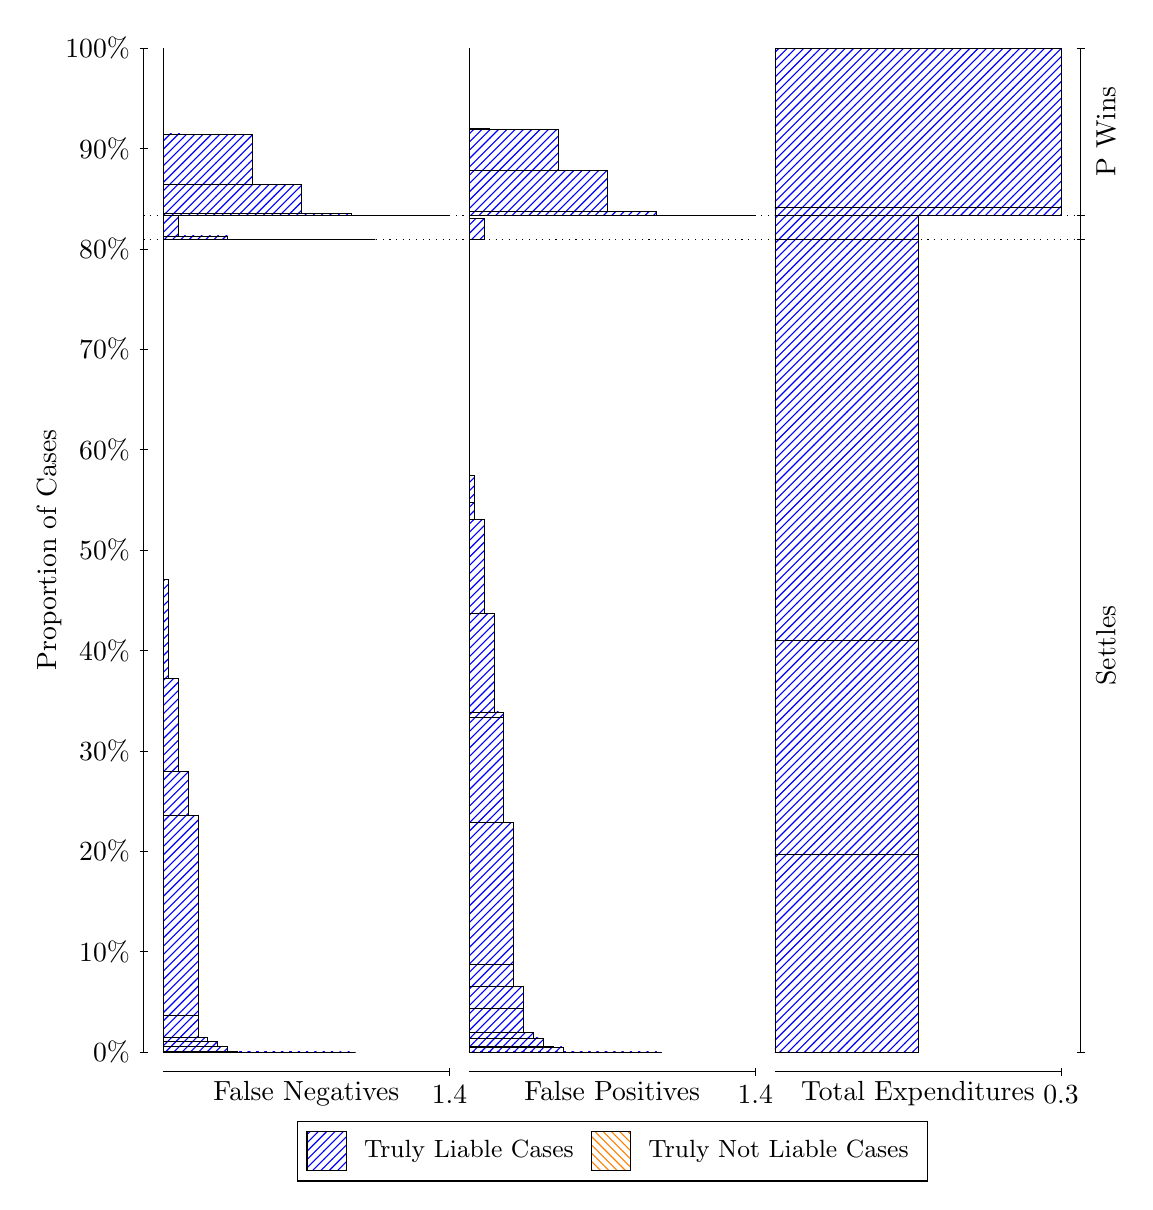
\begin{tikzpicture}
\draw[black, very thin] (1.5,1.75) -- (1.5,14.5);
\node[rotate=90, anchor=center] at (0.3, 8.125) {Proportion of Cases};
\draw[black, very thin] (1.45,1.75) -- (1.55,1.75);
\node[anchor=east] at (1.45, 1.75) {0\%};
\draw[black, very thin] (1.45,3.025) -- (1.55,3.025);
\node[anchor=east] at (1.45, 3.025) {10\%};
\draw[black, very thin] (1.45,4.3) -- (1.55,4.3);
\node[anchor=east] at (1.45, 4.3) {20\%};
\draw[black, very thin] (1.45,5.575) -- (1.55,5.575);
\node[anchor=east] at (1.45, 5.575) {30\%};
\draw[black, very thin] (1.45,6.85) -- (1.55,6.85);
\node[anchor=east] at (1.45, 6.85) {40\%};
\draw[black, very thin] (1.45,8.125) -- (1.55,8.125);
\node[anchor=east] at (1.45, 8.125) {50\%};
\draw[black, very thin] (1.45,9.4) -- (1.55,9.4);
\node[anchor=east] at (1.45, 9.4) {60\%};
\draw[black, very thin] (1.45,10.675) -- (1.55,10.675);
\node[anchor=east] at (1.45, 10.675) {70\%};
\draw[black, very thin] (1.45,11.95) -- (1.55,11.95);
\node[anchor=east] at (1.45, 11.95) {80\%};
\draw[black, very thin] (1.45,13.225) -- (1.55,13.225);
\node[anchor=east] at (1.45, 13.225) {90\%};
\draw[black, very thin] (1.45,14.5) -- (1.55,14.5);
\node[anchor=east] at (1.45, 14.5) {100\%};

\draw[black, very thin] (13.4,1.75) -- (13.4,14.5);
\draw[black, very thin] (13.35,1.75) -- (13.45,1.75);
\node[anchor=west] at (13.35, 1.75) {};
\draw[black, very thin] (13.35,12.072) -- (13.45,12.072);
\node[anchor=west] at (13.35, 12.072) {};
\draw[black, very thin] (13.35,12.376) -- (13.45,12.376);
\node[anchor=west] at (13.35, 12.376) {};
\draw[black, very thin] (13.35,14.5) -- (13.45,14.5);
\node[anchor=west] at (13.35, 14.5) {};

\draw[black, very thin, pattern color=blue, pattern=north east lines] (1.75,1.75) rectangle (4.1931,1.75);
\draw[black, very thin, pattern color=blue, pattern=north east lines] (1.75,1.75) rectangle (3.9425,1.75);
\draw[black, very thin, pattern color=blue, pattern=north east lines] (1.75,1.75) rectangle (3.692,1.75);
\draw[black, very thin, pattern color=blue, pattern=north east lines] (1.75,1.75) rectangle (3.5667,1.75);
\draw[black, very thin, pattern color=blue, pattern=north east lines] (1.75,1.75) rectangle (3.4414,1.75);
\draw[black, very thin, pattern color=blue, pattern=north east lines] (1.75,1.75) rectangle (3.3161,1.75);
\draw[black, very thin, pattern color=blue, pattern=north east lines] (1.75,1.75) rectangle (3.1908,1.75);
\draw[black, very thin, pattern color=blue, pattern=north east lines] (1.75,1.75) rectangle (3.0655,1.75);
\draw[black, very thin, pattern color=blue, pattern=north east lines] (1.75,1.75) rectangle (2.9402,1.75);
\draw[black, very thin, pattern color=blue, pattern=north east lines] (1.75,1.75) rectangle (2.8149,1.7506);
\draw[black, very thin, pattern color=blue, pattern=north east lines] (1.75,1.7506) rectangle (2.6897,1.7551);
\draw[black, very thin, pattern color=blue, pattern=north east lines] (1.75,1.7551) rectangle (2.5644,1.8183);
\draw[black, very thin, pattern color=blue, pattern=north east lines] (1.75,1.8183) rectangle (2.4391,1.8834);
\draw[black, very thin, pattern color=blue, pattern=north east lines] (1.75,1.8834) rectangle (2.4391,1.8834);
\draw[black, very thin, pattern color=blue, pattern=north east lines] (1.75,1.8834) rectangle (2.3138,1.9368);
\draw[black, very thin, pattern color=blue, pattern=north east lines] (1.75,1.9368) rectangle (2.1885,2.2108);
\draw[black, very thin, pattern color=blue, pattern=north east lines] (1.75,2.2108) rectangle (2.1885,4.7525);
\draw[black, very thin, pattern color=blue, pattern=north east lines] (1.75,4.7525) rectangle (2.0632,5.3099);
\draw[black, very thin, pattern color=blue, pattern=north east lines] (1.75,5.3099) rectangle (1.9379,6.4989);
\draw[black, very thin, pattern color=blue, pattern=north east lines] (1.75,6.4989) rectangle (1.8126,7.754);
\draw[black, very thin, pattern color=blue, pattern=north east lines] (1.75,7.754) rectangle (1.8126,7.754);
\draw[black, very thin, pattern color=orange, pattern=north west lines] (1.75,7.754) rectangle (1.75,7.754);
\draw[black, very thin, pattern color=blue, pattern=north east lines] (1.75,7.754) rectangle (1.75,12.072);
\draw[black, very thin, pattern color=blue, pattern=north east lines] (1.75,12.072) rectangle (4.4437,12.072);
\draw[black, very thin, pattern color=blue, pattern=north east lines] (1.75,12.072) rectangle (3.8172,12.072);
\draw[black, very thin, pattern color=blue, pattern=north east lines] (1.75,12.072) rectangle (3.1908,12.072);
\draw[black, very thin, pattern color=blue, pattern=north east lines] (1.75,12.072) rectangle (2.5644,12.113);
\draw[black, very thin, pattern color=blue, pattern=north east lines] (1.75,12.113) rectangle (1.9379,12.376);
\draw[black, very thin, pattern color=orange, pattern=north west lines] (1.75,12.376) rectangle (1.75,12.376);
\draw[black, very thin, pattern color=blue, pattern=north east lines] (1.75,12.376) rectangle (5.3833,12.376);
\draw[black, very thin, pattern color=blue, pattern=north east lines] (1.75,12.376) rectangle (4.7569,12.376);
\draw[black, very thin, pattern color=blue, pattern=north east lines] (1.75,12.376) rectangle (4.1305,12.398);
\draw[black, very thin, pattern color=blue, pattern=north east lines] (1.75,12.398) rectangle (3.504,12.768);
\draw[black, very thin, pattern color=blue, pattern=north east lines] (1.75,12.768) rectangle (3.2534,12.768);
\draw[black, very thin, pattern color=blue, pattern=north east lines] (1.75,12.768) rectangle (2.8776,13.401);
\draw[black, very thin, pattern color=blue, pattern=north east lines] (1.75,13.401) rectangle (2.627,13.401);
\draw[black, very thin, pattern color=blue, pattern=north east lines] (1.75,13.401) rectangle (2.2511,13.408);
\draw[black, very thin, pattern color=blue, pattern=north east lines] (1.75,13.408) rectangle (2.0006,13.411);
\draw[black, very thin, pattern color=orange, pattern=north west lines] (1.75,13.411) rectangle (1.75,13.411);
\draw[black, very thin, pattern color=blue, pattern=north east lines] (1.75,13.411) rectangle (1.75,14.5);
\draw[black, very thin, pattern color=orange, pattern=north west lines] (5.6333,1.75) rectangle (8.0764,1.75);
\draw[black, very thin, pattern color=blue, pattern=north east lines] (5.6333,1.75) rectangle (8.0764,1.75);
\draw[black, very thin, pattern color=orange, pattern=north west lines] (5.6333,1.75) rectangle (7.8259,1.75);
\draw[black, very thin, pattern color=blue, pattern=north east lines] (5.6333,1.75) rectangle (7.8259,1.75);
\draw[black, very thin, pattern color=orange, pattern=north west lines] (5.6333,1.75) rectangle (7.5753,1.75);
\draw[black, very thin, pattern color=blue, pattern=north east lines] (5.6333,1.75) rectangle (7.5753,1.75);
\draw[black, very thin, pattern color=blue, pattern=north east lines] (5.6333,1.75) rectangle (7.45,1.75);
\draw[black, very thin, pattern color=orange, pattern=north west lines] (5.6333,1.75) rectangle (7.3247,1.75);
\draw[black, very thin, pattern color=blue, pattern=north east lines] (5.6333,1.75) rectangle (7.3247,1.75);
\draw[black, very thin, pattern color=blue, pattern=north east lines] (5.6333,1.75) rectangle (7.1994,1.7501);
\draw[black, very thin, pattern color=orange, pattern=north west lines] (5.6333,1.7501) rectangle (7.0741,1.7501);
\draw[black, very thin, pattern color=blue, pattern=north east lines] (5.6333,1.7501) rectangle (7.0741,1.7502);
\draw[black, very thin, pattern color=blue, pattern=north east lines] (5.6333,1.7502) rectangle (6.9489,1.7508);
\draw[black, very thin, pattern color=orange, pattern=north west lines] (5.6333,1.7508) rectangle (6.8236,1.7508);
\draw[black, very thin, pattern color=blue, pattern=north east lines] (5.6333,1.7508) rectangle (6.8236,1.7517);
\draw[black, very thin, pattern color=blue, pattern=north east lines] (5.6333,1.7517) rectangle (6.8236,1.8159);
\draw[black, very thin, pattern color=blue, pattern=north east lines] (5.6333,1.8159) rectangle (6.6983,1.8183);
\draw[black, very thin, pattern color=orange, pattern=north west lines] (5.6333,1.8183) rectangle (6.573,1.8183);
\draw[black, very thin, pattern color=blue, pattern=north east lines] (5.6333,1.8183) rectangle (6.573,1.9281);
\draw[black, very thin, pattern color=blue, pattern=north east lines] (5.6333,1.9281) rectangle (6.4477,1.9949);
\draw[black, very thin, pattern color=orange, pattern=north west lines] (5.6333,1.9949) rectangle (6.3224,1.9949);
\draw[black, very thin, pattern color=blue, pattern=north east lines] (5.6333,1.9949) rectangle (6.3224,2.3041);
\draw[black, very thin, pattern color=blue, pattern=north east lines] (5.6333,2.3041) rectangle (6.3224,2.5804);
\draw[black, very thin, pattern color=blue, pattern=north east lines] (5.6333,2.5804) rectangle (6.1971,2.8579);
\draw[black, very thin, pattern color=blue, pattern=north east lines] (5.6333,2.8579) rectangle (6.1971,4.662);
\draw[black, very thin, pattern color=orange, pattern=north west lines] (5.6333,4.662) rectangle (6.0718,4.662);
\draw[black, very thin, pattern color=blue, pattern=north east lines] (5.6333,4.662) rectangle (6.0718,6.004);
\draw[black, very thin, pattern color=blue, pattern=north east lines] (5.6333,6.004) rectangle (6.0718,6.0677);
\draw[black, very thin, pattern color=blue, pattern=north east lines] (5.6333,6.0677) rectangle (5.9466,7.3227);
\draw[black, very thin, pattern color=blue, pattern=north east lines] (5.6333,7.3227) rectangle (5.8213,8.5118);
\draw[black, very thin, pattern color=blue, pattern=north east lines] (5.6333,8.5118) rectangle (5.696,8.7313);
\draw[black, very thin, pattern color=blue, pattern=north east lines] (5.6333,8.7313) rectangle (5.696,9.0691);
\draw[black, very thin, pattern color=blue, pattern=north east lines] (5.6333,9.0691) rectangle (5.6333,12.072);
\draw[black, very thin, pattern color=orange, pattern=north west lines] (5.6333,12.072) rectangle (5.8213,12.072);
\draw[black, very thin, pattern color=blue, pattern=north east lines] (5.6333,12.072) rectangle (5.8213,12.335);
\draw[black, very thin, pattern color=blue, pattern=north east lines] (5.6333,12.335) rectangle (5.6333,12.376);
\draw[black, very thin, pattern color=orange, pattern=north west lines] (5.6333,12.376) rectangle (9.2667,12.376);
\draw[black, very thin, pattern color=blue, pattern=north east lines] (5.6333,12.376) rectangle (9.2667,12.376);
\draw[black, very thin, pattern color=orange, pattern=north west lines] (5.6333,12.376) rectangle (8.6402,12.376);
\draw[black, very thin, pattern color=blue, pattern=north east lines] (5.6333,12.376) rectangle (8.6402,12.377);
\draw[black, very thin, pattern color=orange, pattern=north west lines] (5.6333,12.377) rectangle (8.0138,12.377);
\draw[black, very thin, pattern color=blue, pattern=north east lines] (5.6333,12.377) rectangle (8.0138,12.421);
\draw[black, very thin, pattern color=orange, pattern=north west lines] (5.6333,12.421) rectangle (7.3874,12.421);
\draw[black, very thin, pattern color=blue, pattern=north east lines] (5.6333,12.421) rectangle (7.3874,12.947);
\draw[black, very thin, pattern color=blue, pattern=north east lines] (5.6333,12.947) rectangle (6.7609,13.465);
\draw[black, very thin, pattern color=orange, pattern=north west lines] (5.6333,13.465) rectangle (6.5103,13.465);
\draw[black, very thin, pattern color=blue, pattern=north east lines] (5.6333,13.465) rectangle (6.5103,13.465);
\draw[black, very thin, pattern color=blue, pattern=north east lines] (5.6333,13.465) rectangle (6.1345,13.468);
\draw[black, very thin, pattern color=orange, pattern=north west lines] (5.6333,13.468) rectangle (5.8839,13.468);
\draw[black, very thin, pattern color=blue, pattern=north east lines] (5.6333,13.468) rectangle (5.8839,13.474);
\draw[black, very thin, pattern color=blue, pattern=north east lines] (5.6333,13.474) rectangle (5.8839,13.475);
\draw[black, very thin, pattern color=orange, pattern=north west lines] (5.6333,13.475) rectangle (5.6333,13.475);
\draw[black, very thin, pattern color=blue, pattern=north east lines] (5.6333,13.475) rectangle (5.6333,14.5);
\draw[black, very thin, pattern color=orange, pattern=north west lines] (9.5167,1.75) rectangle (11.333,1.75);
\draw[black, very thin, pattern color=blue, pattern=north east lines] (9.5167,1.75) rectangle (11.333,4.2619);
\draw[black, very thin, pattern color=orange, pattern=north west lines] (9.5167,4.2619) rectangle (11.333,4.2619);
\draw[black, very thin, pattern color=blue, pattern=north east lines] (9.5167,4.2619) rectangle (11.333,6.9738);
\draw[black, very thin, pattern color=orange, pattern=north west lines] (9.5167,6.9738) rectangle (11.333,6.9738);
\draw[black, very thin, pattern color=blue, pattern=north east lines] (9.5167,6.9738) rectangle (11.333,12.072);
\draw[black, very thin, pattern color=orange, pattern=north west lines] (9.5167,12.072) rectangle (11.333,12.072);
\draw[black, very thin, pattern color=blue, pattern=north east lines] (9.5167,12.072) rectangle (11.333,12.376);
\draw[black, very thin, pattern color=orange, pattern=north west lines] (9.5167,12.376) rectangle (13.15,12.376);
\draw[black, very thin, pattern color=blue, pattern=north east lines] (9.5167,12.376) rectangle (13.15,12.473);
\draw[black, very thin, pattern color=orange, pattern=north west lines] (9.5167,12.473) rectangle (13.15,12.473);
\draw[black, very thin, pattern color=blue, pattern=north east lines] (9.5167,12.473) rectangle (13.15,14.5);
\draw[black, dotted] (1.5,12.072) -- (13.4,12.072);
\draw[black, dotted] (1.5,12.376) -- (13.4,12.376);
\draw[black, very thin] (1.75,1.5) -- (5.3833,1.5);
\node[anchor=north] at (3.5667, 1.5) {False Negatives};
\draw[black, very thin] (5.3833,1.45) -- (5.3833,1.55);
\node[anchor=north] at (5.3833, 1.45) {1.4};

\draw[black, very thin] (5.6333,1.5) -- (9.2667,1.5);
\node[anchor=north] at (7.45, 1.5) {False Positives};
\draw[black, very thin] (9.2667,1.45) -- (9.2667,1.55);
\node[anchor=north] at (9.2667, 1.45) {1.4};

\draw[black, very thin] (9.5167,1.5) -- (13.15,1.5);
\node[anchor=north] at (11.333, 1.5) {Total Expenditures};
\draw[black, very thin] (13.15,1.45) -- (13.15,1.55);
\node[anchor=north] at (13.15, 1.45) {0.3};

\node[black, centered, rotate=90] at (13.72, 6.9108) {Settles};

\node[black, centered, rotate=90] at (13.72, 13.438) {P Wins};

\draw (7.449999999999999,1.5) node[draw=none] (baseCoordinate) {};
\begin{scope}[align=center]
        \matrix[scale=0.5, draw=black, below=0.5cm of baseCoordinate, nodes={draw}, column sep=0.1cm]{
            \node[rectangle, draw, minimum width=0.5cm, minimum height=0.5cm, pattern=north east lines, pattern color=blue] {}; &
            \node[draw=none, font=\small] (B) {Truly Liable Cases}; &
            \node[rectangle, draw, minimum width=0.5cm, minimum height=0.5cm, pattern=north west lines, pattern color=orange] {}; &
            \node[draw=none, font=\small] (B) {Truly Not Liable Cases}; \\
            };
\end{scope}

\end{tikzpicture}
\end{document}